\documentclass[12pt]{jarticle}
\usepackage{TUSIReport}
\usepackage{otf}
\usepackage[dvipdfmx]{graphicx}
\usepackage[dvipdfmx]{color}
\usepackage{amsmath}
\usepackage{amssymb}
\usepackage{color}
\usepackage{hhline}
\usepackage{fancybox,ascmac}
\usepackage{multirow}
\usepackage{url}
\usepackage{bm}
\usepackage{listings,jlisting}
\lstdefinestyle{log}{
    frame={tblr},
    basicstyle={\footnotesize},
    tabsize={4},
}
\lstdefinestyle{lsthtml}{
    language={html},
    backgroundcolor={\color[gray]{.85}},
    basicstyle={\small},
    identifierstyle={\small},
    commentstyle={\small\ttfamily \color[rgb]{0,0.5,0}},
    keywordstyle={\small\bfseries \color[rgb]{1,0,0}},
    ndkeywordstyle={\small},
    stringstyle={\small\ttfamily \color[rgb]{0,0,1}},
    frame={tb},
    breaklines=true,
    columns=[l]{fullflexible},
    numbers=left,
    xrightmargin=0zw,
    xleftmargin=3zw,
    numberstyle={\scriptsize},
    stepnumber=1,
    numbersep=1zw,
    morecomment=[l]{//}
}
\lstdefinestyle{lstphp}{
    language={php},
    backgroundcolor={\color[gray]{.85}},
    basicstyle={\small},
    identifierstyle={\small},
    commentstyle={\small\ttfamily \color[rgb]{0,0.5,0}},
    keywordstyle={\small\bfseries \color[rgb]{1,0,0}},
    ndkeywordstyle={\small},
    stringstyle={\small\ttfamily \color[rgb]{0,0,1}},
    frame={tb},
    breaklines=true,
    columns=[l]{fullflexible},
    numbers=left,
    xrightmargin=0zw,
    xleftmargin=3zw,
    numberstyle={\scriptsize},
    stepnumber=1,
    numbersep=1zw,
    morecomment=[l]{//}
}
\begin{document}
%%%%%%%%%%%%%%%%%%%%%%%%%%%%%%%%%%%%%%%%%%%%%%%%%%%%%%%%%%%%%%
% 表紙を出力する場合は,\提出者と\共同実験者をいれる
% \提出者{科目名}{課題名}{提出年}{提出月}{提出日}{学籍番号}{氏名}
% \共同実験者{一人目}{二人目}{..}{..}{..}{..}{..}{八人目}
%%%%%%%%%%%%%%%%%%%%%%%%%%%%%%%%%%%%%%%%%%%%%%%%%%%%%%%%%%%%%%
\提出者{情報工学実験2}{実験テーマ2 Webアプリケーション}{2020}{10}{5,12}{4619055}{辰川力駆}
\共同実験者{}{}{}{}{}{}{}{}

%%%%%%%%%%%%%%%%%%%%%%%%%%%%%%%%%%%%%%%%%%%%%%%%%%%%%%%%%%%%%%
% 表紙を出力しない場合は,以下の「\表紙出力」をコメントアウトする
%%%%%%%%%%%%%%%%%%%%%%%%%%%%%%%%%%%%%%%%%%%%%%%%%%%%%%%%%%%%%%
\表紙出力

%%%%%%%%%%%%%%%%%%%%%%%%%%%%%%%%%%%%%%%%%%%%%%%%%%%%%%%%%%%%%%
% 以下はレポート本体である.別途 TeXファイルを作成し \input 使っても良い
%%%%%%%%%%%%%%%%%%%%%%%%%%%%%%%%%%%%%%%%%%%%%%%%%%%%%%%%%%%%%%

\section{実験の要旨}
Webアプリケーションとは、
インターネットなどのネットワークを介して、
利用者に対して様々なサービスを提供するアプリケーションのことである。
サービスの要求に対してWebサーバで処理した結果をクライアント側のWebブラウザに表示するため、
アプリケーションをインストールする必要はなく、
クライアント側の環境に頼らずにクロスプラットフォームに対応しているという利点がある。

\section{実験の目的}
本実験では、Webアプリケーションの開発を通じて、
Webアプリケーションの仕組み、オブジェクト指向によるソフトウェア開発の考え方、
データベース管理を理解することを目的とする。

\section{実験の原理}
\subsection{Webアプリケーションの仕組み}
Webアプリケーションでは、アプリケーションに関する処理はほぼすべてサーバで行われる。
このため、アプリケーションに新たな機能が追加された場合や、
新たに別のアプリケーションのサービスを受ける場合などにおいても、
サービスを提供する側のサーバソフトウェアを変更するだけで良く、
利用者側は何も変更することなく新たなサービスが受けられる。

サーバはクライアントからの要求に従い、
HTMLや画像データなどを送信し、
Webブラウザはそのデータを表示する。
サーバは、クライアントからのリクエストを待ち受けており、
クライアントからのリクエストが到着すると処理を行い、
レスポンスを返す。
また、サーバはクライアントからのリクエストを解釈し、
クライアントはサーバの応答を解釈する必要がある。
この要求/応答のやり取りの方式や解釈の方式の取り決めをHTTPと呼ぶ。
以下に処理の概要を示す。
\begin{enumerate}
    \item クライアントからサーバに対して接続を行う。
          すなわち、TCPによるコネクションの確立が行われ、双方のコンピュータ同士で通信が可能となる。
    \item クライアントからサーバに対し、「指定したURLの内容を送れ」という意味の
          要求が送られる。
          URIとは、インターネット上のリソースを示す記述法である。
    \item サーバは要求されたURIに対するデータや、
          サーバプログラムによって処理された結果をクライアントに対して送信する。
          クライアントであるWebブラウザでは、返ってきたデータを画面に表示する。
\end{enumerate}

\clearpage

Webアプリケーションの機能を提供するサーバをWebアプリケーションサーバと呼ぶ。
Webアプリケーションサーバは、その上で複数のサーバプログラムを動作させ、
様々なサービスを提供する。
Webアプリケーションサーバは、通常のWebサーバと同じHTTPを用いてブラウザと通信を行うため、
Webアプリケーションは通常のWWWのコンテンツの閲覧と同様にブラウザを用いて利用することができる。

\subsection{URLの構成}
URLの構造は主に4つに分けられる。
例えばURLが、
\begin{center}
    http://www.riku.co.jp/hoge/tatsukawa.html
\end{center}
の場合について下記に示す。
\begin{enumerate}
    \item http: という部分がプロトコル名である。
          これはインターネットでホームページにアクセスする際に必要な記号である。
          SSL暗号化通信でアクセスする際には、httpの後ろに「s」が付く。
    \item www.riku.co.jp という部分がホスト名+ドメイン名である。
          アクセスするサーバを指定するために必要である。
          ホスト名とは、ネットワーク上のコンピューターにつける識別用の文字列のことで、
          一般的にホームページを管理するコンピューターには「www」が用いられる。
          ドメイン名とは、インターネット上のネットワークを特定するための文字列のことで、
          他のホームページと重複することはない。
    \item hoge という部分がディレクトリ名である。
          サーバ内のフォルダ名とそのフォルダの位置を表す文字列のことである。
    \item tatsukawa.html という部分がファイル名である。

          今回の場合はhogeフォルダの中のtatsukawa.htmlを用いていることを示している。
\end{enumerate}

\clearpage

\subsection{HTTPリクエスト/レスポンス}
HTTPとは、WebサーバとWebクライアントの間でデータの送受信を行うために用いられるプロトコルである。
HTTPのメソッドについては、その用途によってGETとPOSTで使い分ける。

\subsubsection*{GETメソッド}
HTTP通信でサーバから情報を取得する時に使用する。
GETでのサーバへのデータの送信方法として、
リクエストURLの後に?に続いて情報を送信する方式であるクエリストリングがある。
URLの末尾に「?」マークを付け、続けて「名前=値」の形式で記述する。
値が複数あるときは「$\&$」で区切り記述する。

\begin{lstlisting}[style = log]
http://example.com/index.html?name1=value1&name2=value2
\end{lstlisting}

このように送信するデータがアドレスバーに表示されてしまうため、
他人に見られる可能性があるので、
他人に見られたくない情報はGETでは送らない。

\subsubsection*{POSTメソッド}
HTTP通信で、サーバへ情報を登録する時に使用する。
データ量が多い場合、バイナリデータを送信したい場合、
他の人に見られたくない情報を送る場合に利用する。
POSTでサーバにデータを送信する際は、メッセージボディにデータが記述される。

以下に、POSTでのサーバからクライアントへのリクエスト例を示す。

\begin{lstlisting}[style = log]
POST /test/ HTTP/1.1
Host: localhost
Content-Length: 25
Content-Type: application/x-www-form-urlencoded

name1=value1&name2=value2
\end{lstlisting}

上記のように、リクエストヘッダの後に一行、
空行が入り、その後POSTで送信したクエリストリングが、
リクエストボディとしてクライアントからサーバへと送信される。
リクエストボディの長さは、「Content-Length:」という項目で表される。

\clearpage

\begin{lstlisting}[style = log]
HTTP/1.1 200 OK
Content-Type: text/html
Date: Mon, 3 Sep 2017 00:00:00 GMT
Last-Modified: Fri, 1 Sep 2017 00:00:00 GMT
Accept-Ranges: bytes
ETag: "011be787c2f41"
Server: Apache/2.4.27(Unix)

<!DOCTYPE html>
<html>
<head>
<metacharset="utf-8">
<title>Sample</title>
</head>
<body>
<p>Hello!</p>
</body>
</html>
\end{lstlisting}

レスポンスメッセージのメッセージヘッダの1行目はステータスラインであり、
HTTPのバージョン、ステータスコードを表している。
ステータスコードを以下の表に示す。
\begin{table}[htb]
    \begin{center}
        \caption{ステータスコード}
        \begin{tabular}{|l|l|}
            \hline
            ステータスコード & 内容               \\
            \hline
            1xx              & 情報               \\
            2xx              & 成功               \\
            3xx              & リダイレクション   \\
            4xx              & クライアントエラー \\
            5xx              & サーバエラー       \\
            \hline
        \end{tabular}
    \end{center}
\end{table}

残りのヘッダ部分にはリクエスト先のウェブサーバの情報等が記述されている。
メッセージボディ部分が、クライアント側で表示される内容となっている。

\subsection{SQL}
JISでは、「複数の独立した利用者に対して、要求に応じてデータを受け入れ、格納し、
供給するためのデータ構造」と定義されている。
この「複数の独立した利用者に対して、データを受け入れ、格納し、供給する」
を行うシステムをデータベース管理システム(DBMS)と呼ぶ。
大量のデータを扱う際に、高速に効率よくデータを操作(追加、更新、削除)したり、
検索したりすることができる。

現在利用されている多くのデータベース管理システムはリレーショナルデータベース管理システム(RDBMS)である。
リレーショナルデータベースは1つ以上のテーブルで構成され、
テーブルは1つ以上の項目(列)で構成される。各項目についてデータ型を定義する。
データは行単位で扱う。

SQLは、リレーショナルデータベースの定義・操作・検索などをするためにデータベース言語であり、
多くのRDBMSがこの言語に対応している。下記に本実験で使用するSQLの操作一覧を示す。

\begin{table}[htb]
    \begin{center}
        \caption{SQL操作一覧}
        \begin{tabular}{|l|l|}
            \hline
            操作           & SQL文                                                                   \\
            \hline
            テーブルの作成 & {\bf CREATE TABLE} テーブル名 (列名 データ型, 列名 データ型, ...)       \\
            データの検索   & {\bf SELECT} 列名 {\bf FROM} テーブル名 {\bf WHERE} 条件式;             \\
            データの追加   & {\bf INSERT INTO} テーブル名(列名, 列名...) {\bf VALUES} (値, 値, ...); \\
            データの更新   & {\bf UPDATE} テーブル名 {\bf SET} 列名 = 値 {\bf WHERE} 条件式;         \\
            データの削除   & {\bf DELETE FROM} テーブル名 {\bf WHERE} 条件式;                        \\
            \hline
        \end{tabular}
    \end{center}
\end{table}

\subsection{MVCモデルの仕組み}
MVCは、ユーザインターフェースをもつアプリケーションを実装するためのデザインパターンである。
アプリケーションの内部データをユーザが直接参照・編集する情報から分離する。
そのためにアプリケーションを以下の3つの部分に分割する。
\begin{itemize}
    \item[Model]アプリケーションデータ、ビジネスロジック、
          アプリケーションが扱う領域のデータと手続きを表現する要素である。
          ここで、ビジネスロジックとは、
          ビジネスオブジェクトをモデル化したデータベース上のデータに対する処理手順を指す。
    \item [View]グラフや図などの任意の情報表現モデルのデータを取り出してユーザが見るのに
          適した形で表示する要素である。
          すなわちUIへの出力を担当する。
          WebアプリケーションではHTML文書を生成して動的にデータを表示するための部分にあたる。
    \item [Controller]入力を受け取りmodelとviewへの命令に変換する
          ユーザからの入力をモデルへのメッセージへと変換してモデルに伝える要素である。
          すなわちUIからの入力を担当する。
          モデルに変更を引き起こす場合もあるが、直接に描画を行ったり、
          モデルの内部データを直接操作したりはしない。
\end{itemize}

\clearpage

\section{実験装置}
\begin{itemize}
    \item MacBook Pro(16-inch,2019)
          \begin{itemize}
              \item ProductName: Mac OS X
              \item ProductVersion:	10.15.5
              \item BuildVersion: 19F101
              \item プロセッサ: 2.6 GHz 6コアIntel Core i7
              \item メモリ: 16 GB 2667 MHz DDR4
          \end{itemize}
    \item ブラウザ : Google Chrome 86.0.4240.80
\end{itemize}


\section{実験結果・考察}
\subsection{課題1}
\begin{shadebox}
    Slim frameworkとTwigを利用して,以下に示す要件を満たす消費税を自動計算するWebアプリケーションを作成する。
    以下に示す2つのファイルを作成する。
    \begin{itemize}
        \item[・] index.php
        \item[・] templates/tax.html
    \end{itemize}

    動作
    \begin{enumerate}
        \item 金額入力画面を表示(結果の表は表示しない)
        \item 金額と消費税の有無の入力
        \item 金額と消費税の有無を判定し、判定結果を表として表示する
    \end{enumerate}
    ルーティング

    GET  /tax 金額入力画面表示

    POST /tax 消費税計算処理、および、結果表示
\end{shadebox}

\clearpage

\begin{figure}[h]
    \begin{center}
        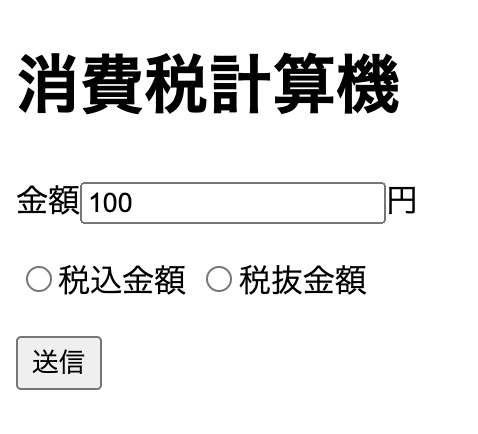
\includegraphics[scale=0.2]{kadai2_1_1.png}
    \end{center}
    \caption{課題1のGETの表示画面}
\end{figure}
図1は初期画面である。tax.htmlの15行目,17行目でinput type=radioにすることにより、
ラジオボダンを実装している。

\begin{figure}[h]
    \begin{minipage}{0.5\hsize}
        \begin{center}
            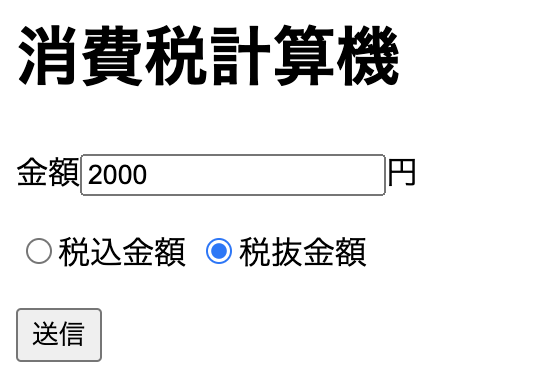
\includegraphics[scale=0.3]{kadai2_1_2.png}
        \end{center}
    \end{minipage}
    \begin{minipage}{0.5\hsize}
        \begin{center}
            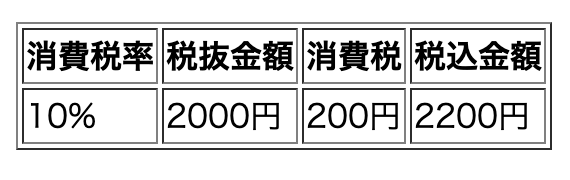
\includegraphics[scale=0.4]{kadai2_1_3.png}
        \end{center}
    \end{minipage}
    \caption{2000円の税抜金額を入力}
\end{figure}
図2は、税抜金額2000円を入力した場合の結果を示す。
index.phpの25行目から28行目では、税抜金額が入力されたならば(data['type']が'extax'ならば)実行をしている。
data['price']で来たものをdata['extax']として消費税を計算している。
\begin{figure}[h]
    \begin{minipage}{0.5\hsize}
        \begin{center}
            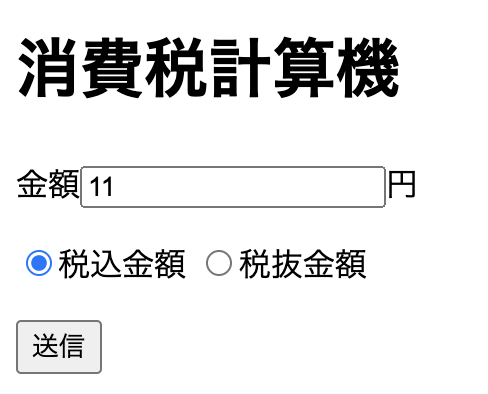
\includegraphics[scale=0.3]{kadai2_1_4.png}
        \end{center}
    \end{minipage}
    \begin{minipage}{0.5\hsize}
        \begin{center}
            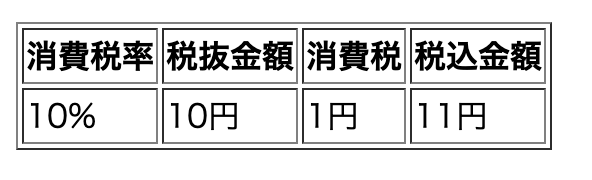
\includegraphics[scale=0.4]{kadai2_1_5.png}
        \end{center}
    \end{minipage}
    \caption{11円の税込金額を入力}
\end{figure}

図3は、税込金額11円を入力した場合の結果を示す。
index.phpの21行目から24行目では、税込金額が入力されたならば(data['type']が'intax'ならば)実行をしている。
data['price']で来たものをdata['intax']として消費税を計算している。

また、GETとPOSTで結果を表示させるかどうかを判定するのは、
tax.htmlの26行目でtaxrateが存在($\neq 0$)すれば、表を出力している。

\clearpage

\subsection{課題2}
\begin{shadebox}
    以下に示す要件を満たす自動販売機のWebアプリケーションを作成する。
    アプリケーションの作成にあたりSlimとTwigを利用し、以下に示す2つのファイルを作成する。

    \begin{itemize}
        \item[・] index2.php
        \item[・] templates/machine.html
    \end{itemize}
    \begin{itemize}
        \item データベース({\bf Model})\\
              列名は,``ID,商品名,価格,数量"とする.\\
              データベースファイル名は、``vending.db"とする
              \newpage
        \item 動作
              \begin{enumerate}
                  \item 商品一覧を表示
                  \item 投入金額、商品の購入個数の入力
                  \item 購入金額と投入金額を判定し、判定結果に応じた処理を行う
                        \begin{itemize}
                            \item (購入可能)

                                  (a) データベースを更新
                                  (b) 結果表示領域にレシート(購入商品、合計金額、おつり)を表示

                            \item(購入不可)結果表示領域に「投入金額不足」を表示
                        \end{itemize}
              \end{enumerate}
              ルーティング

              GET /vending 商品一覧表示

              POST /vending 商品購入処理、および、結果表示
    \end{itemize}
\end{shadebox}

\begin{figure}[h]
    \begin{center}
        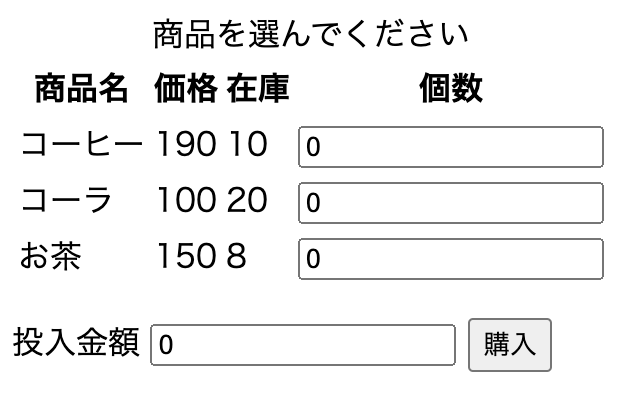
\includegraphics[scale=0.2]{kadai2_2_1.png}
    \end{center}
    \caption{課題2のGETの表示画面}
\end{figure}
図4は初期画面である。初期のmachine.htmlとほぼ変わりはない。
ただし、細かいことだが投入額を投入金額に変えている。

\clearpage

\begin{figure}[h]
    \begin{minipage}{0.5\hsize}
        \begin{center}
            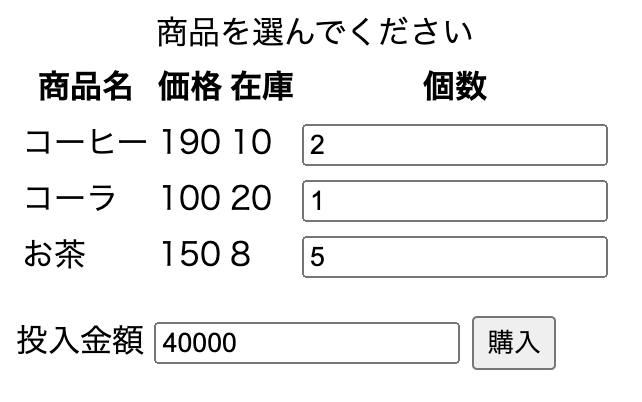
\includegraphics[scale=0.4]{kadai2_2_2.png}
        \end{center}
    \end{minipage}
    \begin{minipage}{0.5\hsize}
        \begin{center}
            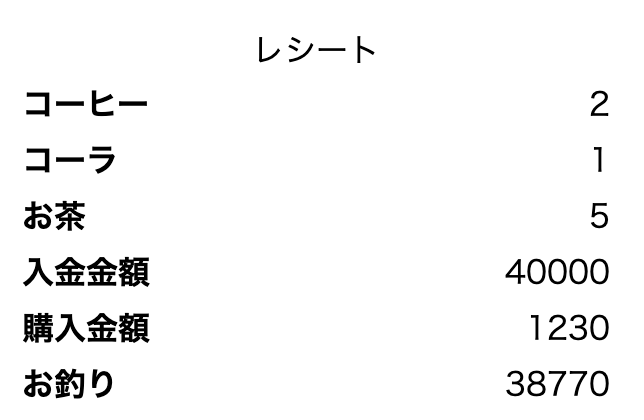
\includegraphics[scale=0.4]{kadai2_2_3.png}
        \end{center}
    \end{minipage}
    \caption{正しい入力がされた場合の結果}
\end{figure}

図5は正しい入力がされた場合の結果を表示している。
index.phpの78行目でエラーが1つもない場合は、79行目でdata['result']を'Finish'にして、
80行目以降でデータベースを更新している。

data['result']を'Finish'にすることにより、
machine.htmlの37行目のif文で'Finish'ならばレシートを表示している。

図6以降は、エラー処理についてまとめたものである。
また、エラーの出力はmachine.htmlの63行目で
data['result']が'Error'ならば、for文でエラーを一つ一つ表示している。
\begin{figure}[h]
    \begin{minipage}{0.5\hsize}
        \begin{center}
            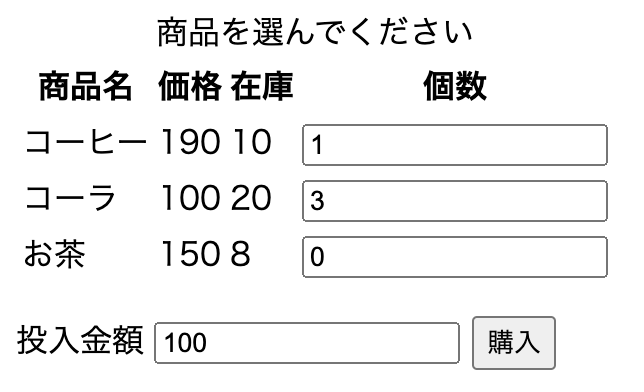
\includegraphics[scale=0.4]{kadai2_2_4.png}
        \end{center}
    \end{minipage}
    \begin{minipage}{0.5\hsize}
        \begin{center}
            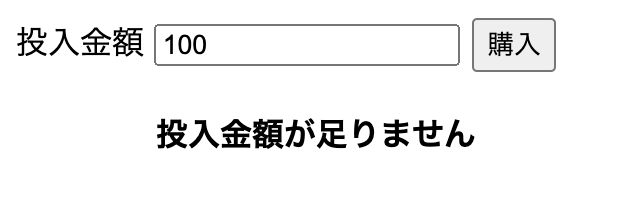
\includegraphics[scale=0.4]{kadai2_2_5.png}
        \end{center}
    \end{minipage}
    \caption{投入金額が足りなかった場合の結果}
\end{figure}

図6は、投入金額が足りなかった場合の結果を表示している。
課題2のindex.phpの72行目から76行目で実装している。
$入力された金額-支払総額$が負の場合はエラー処理をしている。
\clearpage

\begin{figure}[h]
    \begin{minipage}{0.5\hsize}
        \begin{center}
            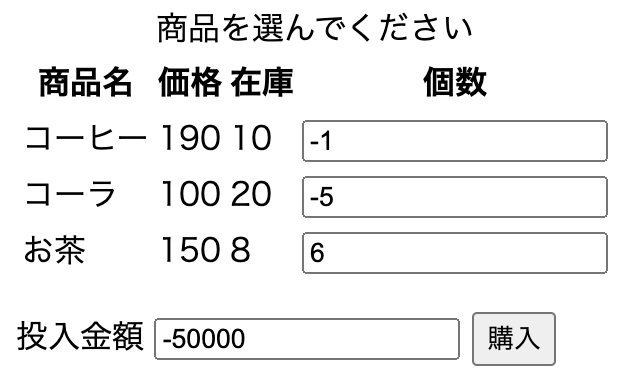
\includegraphics[scale=0.4]{kadai2_2_6.png}
        \end{center}
    \end{minipage}
    \begin{minipage}{0.5\hsize}
        \begin{center}
            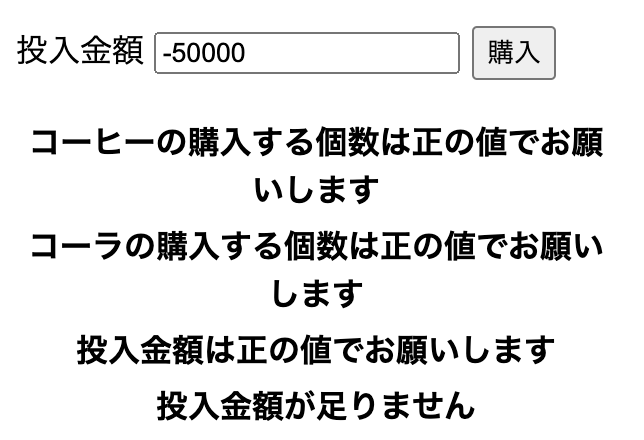
\includegraphics[scale=0.4]{kadai2_2_7.png}
        \end{center}
    \end{minipage}
    \caption{負の値が入力された場合の結果}
\end{figure}

図7は、負の値が入力された場合の結果を表示している。
課題2のindex.phpの56行目から60行目では、購入する個数が負の値の場合を実装している。
支払う金額が負の値の場合の実装は64行目から68行目である。
どちらも、0より少なければエラー処理を施しただけである。
\begin{figure}[h]
    \begin{minipage}{0.5\hsize}
        \begin{center}
            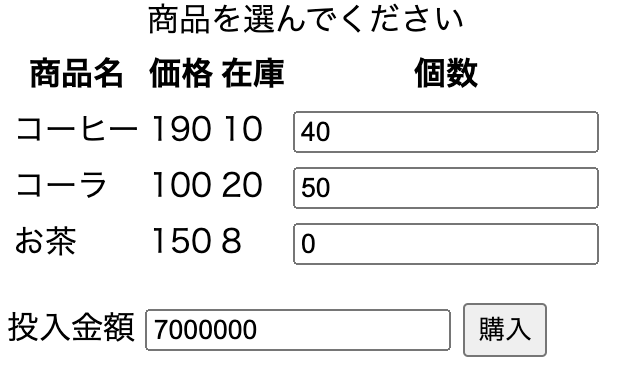
\includegraphics[scale=0.4]{kadai2_2_8.png}
        \end{center}
    \end{minipage}
    \begin{minipage}{0.5\hsize}
        \begin{center}
            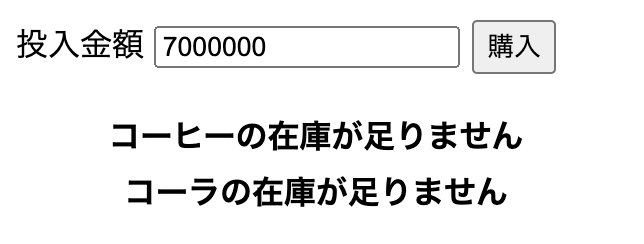
\includegraphics[scale=0.4]{kadai2_2_9.png}
        \end{center}
    \end{minipage}
    \caption{在庫が足りない場合の結果}
\end{figure}

図8は、在庫が足りない場合の結果を表示している。
課題2のindex.phpの51行目から55行目で実装している。
$入力された個数>在庫$ならばエラー処理をしている。

\clearpage

\begin{figure}[h]
    \begin{minipage}{0.5\hsize}
        \begin{center}
            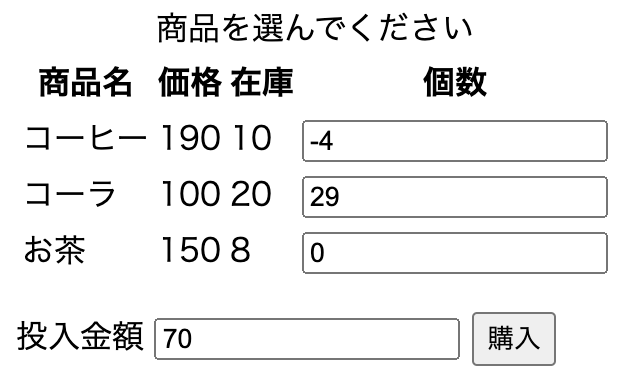
\includegraphics[scale=0.4]{kadai2_2_10.png}
        \end{center}
    \end{minipage}
    \begin{minipage}{0.5\hsize}
        \begin{center}
            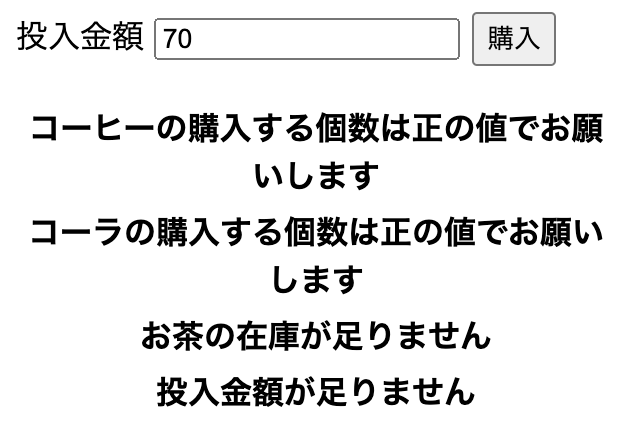
\includegraphics[scale=0.4]{kadai2_2_11.png}
        \end{center}
    \end{minipage}
    \caption{複数のエラーが出力された場合の結果}
\end{figure}

図9は、複数のエラーが出力された場合の結果を表示している。
これは、いままでのエラーハンドリングの実装のまとめである。
複数のエラーを出力できているのは、index.phpの47行目で用意したエラーの数を数える変数data['count']を用意することで、
エラーが発見される度にdata['errorlog'][data['count']]にエラーを入れてcountをプラス1しているからである。

\subsection{フレームワークのメリット・デメリット}
\subsubsection*{メリット}
機能やデザインのカスタマイズが容易にできる。
また、短時間で高品質なアプリケーションを開発することが可能である。
さらに、コードの統一性が生まれ、コードが見やすくなる。

\subsubsection*{デメリット}
言語の勉強以外に、その言語のフレームワークも勉強しないといけない。
また、費用がかかるものも存在する。

\subsubsection*{フレームワークそれぞれにもメリット・デメリットが存在する}
自分が知っているもので例をあげると、
Go言語のフレームワークには有名なものでEcho,Gin,Beegoなどがあるが、
Beegoは簡単にWebアプリ開発ができ初学者におすすめで、Ginは歴史が古く軽量であり、
EchoはRESTの原則に則っているなどの個別の特徴があります。
\section{まとめ}
今実験では、html,php,SQLiteを用いてWebアプリケーション開発を行った。
Webアプリケーションの開発を通じて、Webアプリケーションの仕組み、
オブジェクト指向によるソフトウェア開発の考え方、
データベース管理を理解することができた。
\clearpage

% 参考文献
\begin{thebibliography}{99}
    \label{sannkoubunnkenn_chapter}
    \bibitem[1]{rikadai}東京理科大学工学部情報工学科 情報工学実験2 2020年度
    東京理科大学工学部情報工学科出版

    \bibitem[2]{toukei}
    分かりやすいURL構造を設計しよう「ディレクトリ名・ファイル名の付け方」 : ビジネスとIT活用に役立つ情報

    \url{https://www.asobou.co.jp/blog/web/url-optimisation}

    最終閲覧日2020/10/18
\end{thebibliography}


\clearpage

% 付録
\appendix
\section{付録}
\begin{lstlisting}[style = lsthtml,caption=tax.html]
<!DOCTYPE html>
<html lang="ja">

<head>
    <meta charset="utf-8">
    <title>消費税計算機</title>
</head>

<body>
    <h1>消費税計算機</h1>
    <form action="" method="POST">
        <p><label>金額<input type="number" name="price" value={{price}}>円
        </label></p>
        <p>
            <label><input type="radio" name="type" value="intax">税込金額
            </label>
            <label><input type="radio" name="type" value="extax">税抜金額
            </label>
        </p>

        <p><input type="submit" value="送信"></p>
    </form>


    <!--$data['taxrate']=10(%)が存在するなら表を表示-->
    
    <table border="1">
        <tr>
            <th>消費税率</th>
            <th>税抜金額</th>
            <th>消費税</th>
            <th>税込金額</th>
        </tr>
        <tr>
            <td>{{taxrate}}%</td>
            <td>{{extax}}円</td>
            <td>{{tax}}円</td>
            <td>{{intax}}円</td>
        </tr>
    </table>
    


</body>

</html>
\end{lstlisting}

\clearpage

\begin{lstlisting}[style = lstphp,caption=課題1のindex.php]
    <?php
    require 'vendor/autoload.php';
    
    $app = new \Slim\App();
    
    $loader = new Twig_Loader_Filesystem('templates');
    $twig = new Twig_Environment($loader);
    
    $app->get('/tax', function ($request, $response, $args) use ($twig) {
        $data = [];
        $data['price'] = 100;
        $html = $twig->render('tax.html', $data);
        return $response->write($html);
    });
    
    //POST "/tax" 税金を計算
    $app->post('/tax', function ($request, $response, $args) use ($twig) {
        $data = $request->getParsedBody();
        $data['rate'] = 0.10;
    
        if ($data['type'] == 'intax') {   //入力されたものが税込金額のとき
            $data['intax'] = $data['price'];
            $data['extax'] = floor($data['intax'] / (1 + $data['rate'])); 
            $data['tax'] = $data['intax'] - $data['extax'];
        } elseif ($data['type'] == 'extax') {  //入力されたものが税抜金額のとき
            $data['extax'] = $data['price'];
            $data['intax'] = floor($data['price'] * (1 + $data['rate']));
            $data['tax'] = $data['intax'] - $data['extax'];
        } else { //エラー
            echo "Error...";
        }
    
        $data['taxrate'] = $data['rate'] * 100;
    
        $html = $twig->render('tax.html', $data);
        return $response->write($html);
    });
    
    $app->run();
    
    \end{lstlisting}

\clearpage
\begin{lstlisting}[style = lsthtml,caption=machine.html]
    <!DOCTYPE html>
    <html lang="ja">
    
    <head>
        <meta charset="utf-8">
        <title>自動販売機</title>
    </head>
    
    <body>
        <form action="" method="POST">
            <table>
                <caption>商品を選んでください</caption>
                <tr>
                    <th>商品名</th>
                    <th>価格</th>
                    <th>在庫</th>
                    <th>個数</th>
                </tr>
                
                <tr>
                    <td>{{item.name}}</td>
                    <td>{{item.price}}</td>
                    <td>{{item.num}}</td>
                    <td><input type="number" name="buyitem[{{item.id}}]" value="0"></td>
                </tr>
                
            </table>
            <p>
                <label>
                    投入金額
                    <input type="number" name="pay" value="{{pay}}">
                    <input type="submit" value="購入">
                </label>
            </p>
        </form>
    
        
        <table width="300">
            <caption>レシート</caption>
            
            
            <tr>
                <th align="left">{{item.name}}</th>
                <td align="right">{{buyitem[item.id]}}</td>
            </tr>
            
            
            <tr>
                <th align="left">入金金額</th>
                <td align="right">{{pay}}</td>
            </tr>
            <tr>
                <th align="left">購入金額</th>
                <td align="right">{{sum}}</td>
            </tr>
            <tr>
                <th align="left">お釣り</th>
                <td align="right">{{change}}</td>
            </tr>
        </table>
        
    
        
        <table width="300">
            
            <tr>
                <th>{{log}}</th>   <!--エラーを出力-->
            </tr>
              
        </table>
        
    </body>
    
    </html>
    \end{lstlisting}

\clearpage
\begin{lstlisting}[style = lstphp,caption=課題2のindex.php]
    <?php
    require 'vendor/autoload.php';
    
    // データベース接続
    try {
        $pdo = new PDO('sqlite:vending.db');
    } catch (PDOException $e) {
        die("データベース接続失敗" . $e->getMessage());
    }
    // テーブル作成
    $pdo->exec("create table if not exists items (
        id    integer primary key autoincrement,
        name  varchar,
        price integer,
        num   integer)");
    
    // SLIM framework の準備
    $app = new \Slim\App();
    
    // twig の準備
    $loader = new Twig_Loader_Filesystem('templates');
    $twig = new Twig_Environment($loader);
    
    //----------------------------------
    // ルーティング
    //----------------------------------
    $app->get('/vending', function ($request, $response, $args) use ($twig, $pdo) {
        $data = [];
        $data['pay'] = 0;
    
        $stmt = $pdo->prepare("SELECT * FROM items");
        $stmt->execute();
        $data['items'] = $stmt->fetchALL();
    
        $html = $twig->render('machine.html', $data);
        return $response->write($html);
    });
    
    $app->post('/vending', function ($request, $response, $args) use ($twig, $pdo) {
        $data = $request->getParsedBody();
    
        $stmt = $pdo->prepare("SELECT * FROM items");
        $stmt->execute();
        $data['items'] = $stmt->fetchALL();
    
        $data['sum'] = 0; //購入する商品の合計金額
        $data['count'] = 0; //エラーの数を数える
    
    
        foreach ($data['items'] as $item) { //items内のitemそれぞれに対して実行
            if ($data['buyitem'][$item['id']] > $item['num']) { //在庫が足りない場合
                $data['result'] = 'Error';
                $data['errorlog'][$data['count']] = sprintf("%sの在庫が足りません", $item['name']);
                $data['count']++;
            }
            if ($data['buyitem'][$item['id']] < 0) { //購入する個数が負の値の場合
                $data['result'] = 'Error';
                $data['errorlog'][$data['count']] = sprintf("%sの購入する個数は正の値でお願いします", $item['name']);
                $data['count']++;
            }
    
            $data['sum'] += $item['price'] * $data['buyitem'][$item['id']];
        }
        if ($data['pay'] < 0) { //投入金額が負の値の場合
            $data['result'] = 'Error';
            $data['errorlog'][$data['count']] = sprintf("投入金額は正の値でお願いします");
            $data['count']++;
        }
    
        $data['change'] = $data['pay'] - $data['sum']; //お釣りを計算
    
        if ($data['change'] < 0) { //お金が足りていない場合
            $data['result'] = 'Error';
            $data['errorlog'][$data['count']] = sprintf("投入金額が足りません");
            $data['count']++;
        }
    
        if ($data['count'] == 0) { //エラーが1つもない場合はsqlのデータベースをupdateする
            $data['result'] = 'Finish';
            foreach ($data['buyitem'] as $key => $num) {
                $sql = "UPDATE items SET num = num - :buy WHERE id = :idkey";
                $stmt = $pdo->prepare($sql);
                $params = array(':buy' => $num, ':idkey' => $key);
                $stmt->execute($params);
            }
    
            $stmt = $pdo->prepare("SELECT * FROM items");
            $stmt->execute();
            $data['items'] = $stmt->fetchALL();
        }
    
        $html = $twig->render('machine.html', $data);
        return $response->write($html);
    });
    
    
    $app->get('/insert/{name}/{num}', function ($request, $response, $args) use ($twig, $pdo) {
        $stmt = $pdo->prepare("insert into items (name, price, num) values (?,?,?)");
        $stmt->execute([$args['name'], 0, $args['num']]);
    
        return $response->write('新商品' . $args['name'] . 'を' . $args['num'] . '個追加しました');
    });
    
    $app->run();
    
    \end{lstlisting}















%%%%%%%%%%%%%%%%%%%%%%%%%%%%%%%%%%%%%%%%%%%%%%%%%%%%%%%%%%%%%%
\end{document}